\documentclass{article}
\usepackage[a4paper,top=2cm,bottom=2cm,left=2cm,right=2cm]{geometry}
\usepackage[english]{babel}
\usepackage{fontenc}
\usepackage[utf8]{inputenc}
\usepackage{fancyhdr}
\usepackage{float}
\usepackage{graphicx}
\usepackage{wrapfig}
\usepackage{siunitx} %per scrivere il simbolo °
\usepackage{verbatim} %per i commenti1
\usepackage{subfig}
\usepackage{amsmath}
\usepackage{algorithm}
\usepackage{algpseudocode}
\setcounter{secnumdepth}{3}
\setcounter{tocdepth}{6}
\usepackage{multirow}
\newcommand{\minitab}[2][l]{\begin{tabular}#1 #2\end{tabular}}
\usepackage{rotating}
\usepackage{xfrac}
\usepackage{cite}

\DeclareMathOperator*{\argmax}{arg\,max}
\DeclareMathOperator*{\argmin}{arg\,min}

%\usepackage{booktabs,array}
%\usepackage{tikz}

%\usepackage{tabularx}

%\usepackage{chngcntr}
%\counterwithin{table}{section}

%------------------------------ colors
\usepackage[usenames,dvipsnames,table]{xcolor} % use colors on table and more
\definecolor{333}{RGB}{51, 51, 51} % define custom color
\definecolor{background}{RGB}{248, 248, 255}
\definecolor{comment}{RGB}{17,167,5}
\definecolor{keyword}{RGB}{195,47,8}
\definecolor{string}{RGB}{142,195,0}
\definecolor{number}{RGB}{90,84,84}
\definecolor{identifier}{RGB}{0,90,201}

%------------------------------ source code
\usepackage{listings}

\lstset{
  basicstyle=\footnotesize\sffamily,
  commentstyle=\itshape\color{gray},
  captionpos=b,
  frame=shadowbox,
  language=HTML,
  rulesepcolor=\color{333},
  tabsize=2
}

\newcommand{\e}[1]{\cdot 10^{#1}}

\title{\textbf{Report about Lab2}} % Title
\author{Raffaele \textsc{Di Nardo Di Maio} 1204879} % Author name
\date{\today}

\begin{document}
\begin{minipage}{.20\textwidth}
  
\includegraphics[height=3cm]{../Icon4}
\end{minipage}\begin{minipage}{.20\textwidth}
  \begin{table}[H]
  \begin{tabular}{l}
  \scshape{\Large{Computer Engineering Master Degree}} \\
  \hline \\
  \scshape{\Large{Computer Vision}} \\
  \end{tabular}
  \end{table}
\end{minipage}
{\let\newpage\relax\maketitle}
\section{Goal of the experience}
The goal of the Lab2 was to calibrate a camera, using a set of images of the same checkerboard, each one with differenct aspect, taken with the same camera. Each image represents the chessboard at a different distance from the camera and with a different orientation in the space. After generating the calibration parameters of the used camera, the goal to find best and worst input images in terms of mean reprojection error. The last thing to do, was the rectification of an image,representing a room and taken by the same camera, by using the parameters estimated previously.
\section{Organization of code}
The code of this lab is organized in four main files:
\begin{itemize}
\item{\textbf{Lab2.cpp} and its header file \textbf{Lab2.h}\\
they are associated to the \textit{main()} and to a function, used to print info about read input files;}
\item{\textbf{Calibration.cpp} and its header file \textbf{Calibration.h}\\
these contain the function \textit{calibrate()} that, using other functions performs checkerboard corners detection on input images and rectifies the test image.}
\end{itemize}
\section{Command line parameters}
The program needs to have, as command line arguments, in order, the specification of the path of checkerboards images folder and the path of test images folder. For example, the sequence of command line arguments, considering "data/checkerboard\_images" as folder of chessboard input images and "data" as folder of test images is:\\
\begin{center}
\begin{tabular}{c}
\begin{lstlisting}[linewidth=160pt, basicstyle=\footnotesize\sffamily,] 
data/checkerboard_images   data
\end{lstlisting}
\end{tabular}
\end{center}
\section{Experimental results}
In the extraction of corners from the input images, I've tried two approaches to compute them. They give me different parameters and mean reprojection errors (see Table \ref{calib} and Table \ref{mean}):
\begin{enumerate}
\item{Direct computation through cv::findChessboardCorners() function}
\item{Improvement of corners precision of first approach using cv::cornerSubPix()\\}
\end{enumerate}
\begin{table}[h]
\centering
\begin{tabular}{|c|l|l|l|}
\cline{3-4}
\multicolumn{1}{c}{}&\multicolumn{1}{c|}{}&{\textbf{Approach 1}}&{\textbf{Approach 2}}\\
\hline
\multirow{4}{*}{Intrinsic parameters}&{$\alpha_u$}&{1245.72}&{1245.11}\\
\cline{2-4}
&{$\alpha_u$}&{1245.19}&{1244.22}\\
\cline{2-4}
&{$u_c$}&{978.874}&{974.987}\\
\cline{2-4}
&{$v_c$}&{686.44}&{684.104}\\
\hline
\multirow{3}{*}{Radial distortion}&{$k_1$}&{-0.3085}&{-0.308478}\\
\cline{2-4}
&{$k_2$}&{0.139678}&{0.138993}\\
\cline{2-4}
&{$k_3$}&{-0.0367748}&{-0.036138}\\
\hline
\multirow{2}{*}{Tangential Distortion}&{$p_1$}&{$5.86927\e{-6}$}&{$-9.79746\e{-5}$}\\
\cline{2-4}
&{$p_2$}&{$7.81765\e{-6}$}&{$3.00305\e{-4}$}\\
\hline
\end{tabular}
\caption{Estimated calibration parameters.}\label{calib}
\end{table}
\begin{table}[h]
\centering
\begin{tabular}{|c|l|l|}
\cline{2-3}
\multicolumn{1}{c|}{}&{\textbf{Approach 1}}&{\textbf{Approach 2}}\\
\hline
{Average of mean reprojection}&\multirow{2}{*}{0.516669}&\multirow{2}{*}{0.294035}\\
{errors of all images}&&\\
\hline
\multirow{2}{*}{Worst image}&{0027\_color.png}&{0045\_color.png}\\
&{Error: 1.54774}&{Error: 1.91905}\\
\hline
\multirow{2}{*}{Best image}&{0002\_color.png}&{0039\_color.png}\\
&{Error: 0.226561}&{Error: 0.0727016}\\
\hline
\end{tabular}
\caption{Mean reprojection errors with 2 approaches.}\label{mean}
\end{table}
\vspace{6cm}
The program also has some commented pieces that I've used to compute and store on disk all checkerboards images, with highlighted chessboard corners(e.g. Figure \ref{chess::best} and Figure \ref{chess::best}), and also final image with comparison between original image and rectified image (see Figure \ref{originVSrect}).\\
For Approach 2, the image in Figure \ref{chess::best} is better than the one in \ref{chess::worst}, in terms of mean reprojection error, because of the angle of chessboard, with respect to the space, and the smoothness of the image.\\
\begin{figure}[h]
\begin{center}
  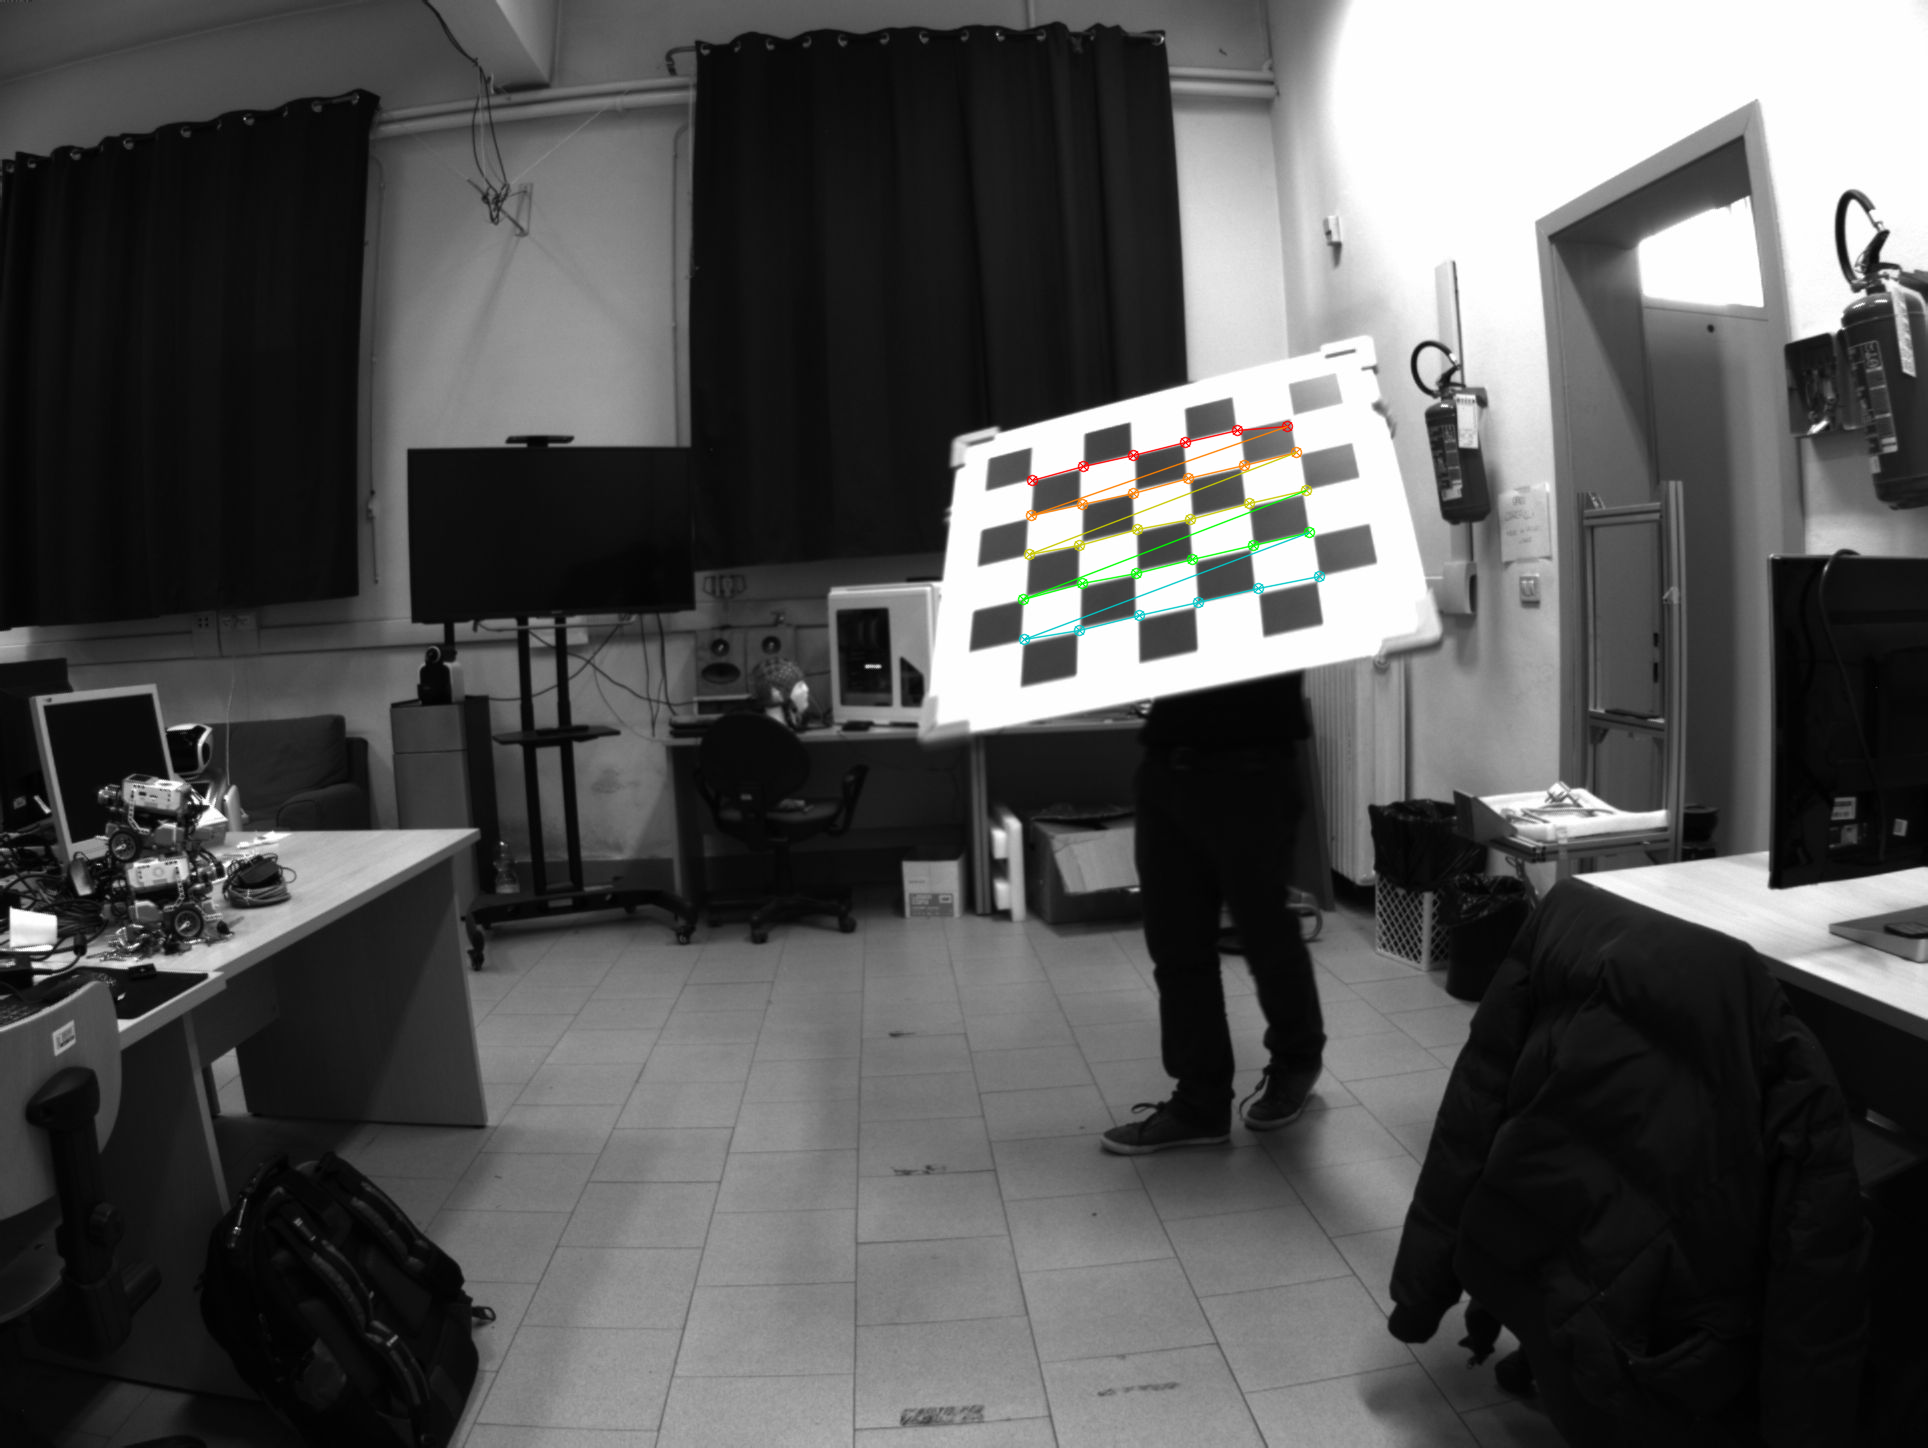
\includegraphics[scale=0.17]{chessboard44}\\ 
  \caption{\footnotesize{Worst image for Approach 2 in terms of mean reprojection error.}}\label{chess::worst} 
\end{center} 
\end{figure}
\begin{figure}[h]
\begin{center} 
  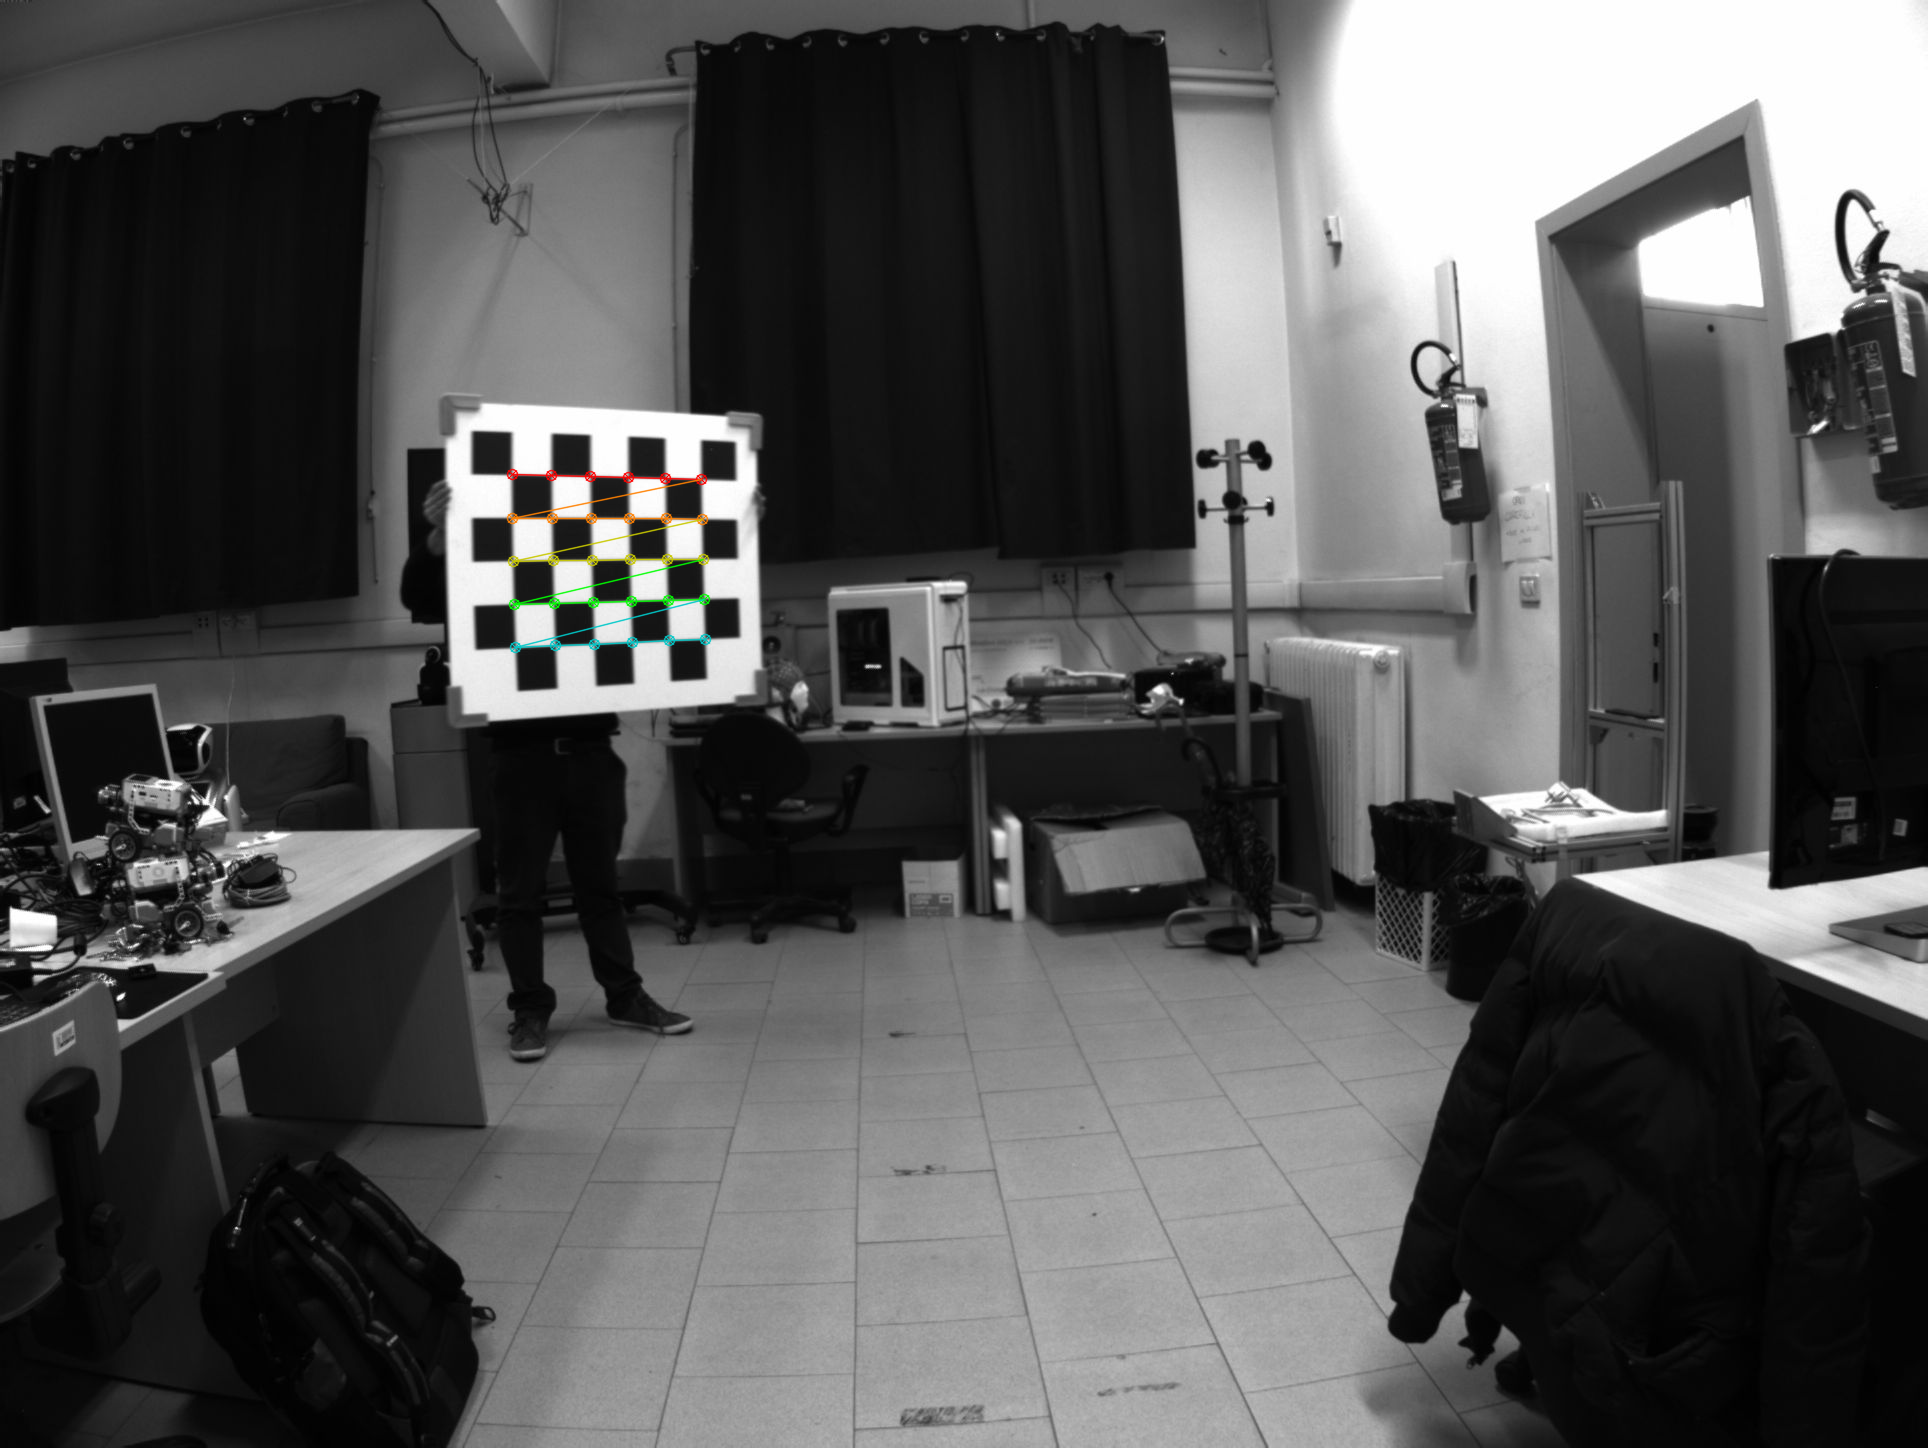
\includegraphics[scale=0.17]{chessboard38}\\ 
  \caption{\footnotesize{Best image for Approach 2 in terms of mean reprojection error.}}
  \label{chess::best} 
\end{center} 
\end{figure}
\begin{figure}[h] 
\begin{center} 
  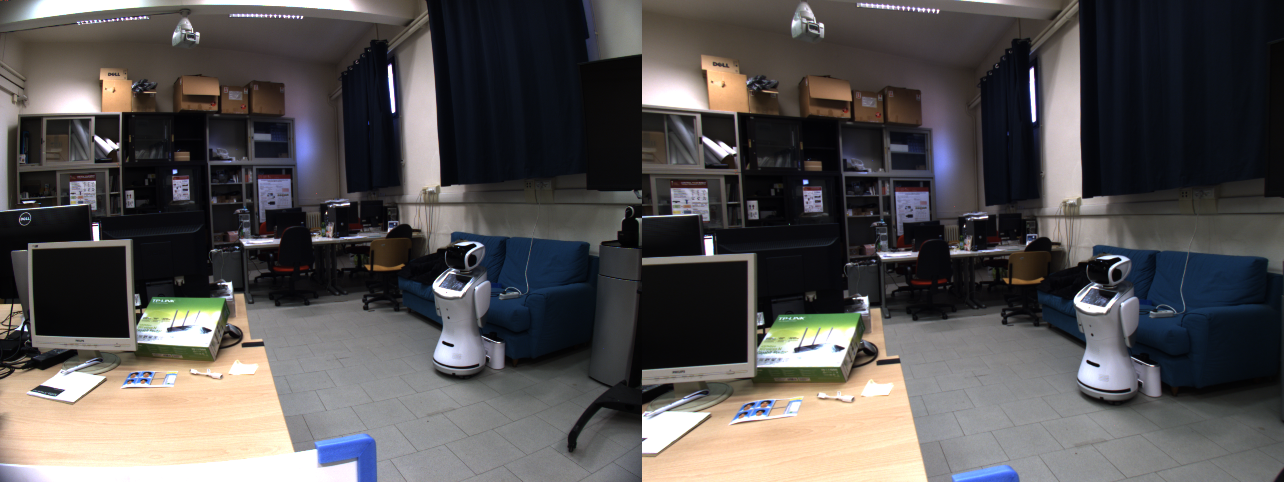
\includegraphics[scale=0.35]{comparison1}\\ 
  \caption{\footnotesize{Original test image (on the left) vs Rectified image (on the right).}}
  \label{originalVSrect} 
\end{center} 
\end{figure}

\end{document}